\documentclass[a4paper]{article}
\usepackage[a4paper, total={6in, 10in}]{geometry}

\usepackage[english]{babel}
\usepackage[utf8]{inputenc}
\usepackage{amsmath}
\usepackage{graphicx}
\usepackage{float}
\usepackage[colorinlistoftodos]{todonotes}
\usepackage[normalem]{ulem}
\usepackage{xcolor}
\usepackage{wrapfig}


\newtheorem{theorem}{Theorem}[section]
\newtheorem{lemma}[theorem]{Lemma}


% usage :
% \myfig[float params]{figure caption}{reference fig:fig1}{figure contents}
\newcommand{\myfig}[4][]{%
% First arg is the float args
	\ifthenelse { \equal {#1}{}}  %
		{\def\flt {\begin{figure}[!ht]}} % #1 is blank
		{\def\flt {\begin{figure}[#1]}} % #1 is not blank
	\flt
	\centering
	#4
	\caption{#2}
	\label{#3}
	\end{figure}
}

% usage:
% \mytable[float placement]{table caption}{label reference ie tab:table1}{table contents}
\newcommand{\mytable}[4][]{%
% First arg is the float args
	\ifthenelse { \equal {#1}{}}  % The float placement
		{\def\tflt {\begin{table}[!ht]}} % #1 is blank
		{\def\tflt {\begin{table}[#1]}} % #1 is not blank
	\tflt
	\centering
	
	#4
	\caption{#2}
	\label{#3}
	\end{table}
}


\title{Fair Stable Marriage - Term Project\\Social Computing - Fall 2018}

\author{Swapna Mukrappilly\\Jason Trout\\Zach Southwell\\Joshua Musick}

\date{\today}

\begin{document}
\maketitle

\begin{abstract}
We explore the problem of finding an optimal stable marriage that considers the overall satisfaction of both men and women and present a reasonable solution to finding this optimal matching.

\end{abstract}

\section{Introduction}
\label{sec:introduction}

\subsection{Stable Marriage Problem}
The Stable Marriage Problem can be described as follows: We are given a set of unmarried men and women. The cardinality of each gender in this set is equal. Each person in this set provides an ordered preference list which contains all members of the opposite gender. We want to produce a matching such that:
\begin{itemize}
    \item Each member of the set is matched with a member of the opposite gender.
    \item There are no blocking pairs. That is to say, there are no two pairs such that the man in one pair and the woman in another pair both prefer each other to their current partners.
\end{itemize}
As shown by Gale and Shapely \cite{shapely}, there is always at least one stable matching to this problem.

The Gale-Shapely algorithm is effective in finding a stable matching given any valid problem set. An interesting property of this algorithm is that it is strongly biased in favor of one of the genders. For the optimal group, each and every member of that group is guaranteed to be matched with the best possible partner for any stable matching. Alternately, each member of the non-optimal group is guaranteed to be matched with the worst possible partner for any stable matching.

\subsection{Fair Matching}
The systematic bias that the Gale-Shapely algorithm applies toward the optimal group is clearly not optimized for fairness. How can we find a more equitable solution?

First, it is important to define what property we are looking for in this solution. Let the function $score(p, m)$ be defined as the position of a person $p$'s assigned match $m$ in their preference list. So for example, if a man $M_1$ has the preference list [$W_3$, $W_1$, $W_4$, $W_2$], and ($M_1$, $W_3$) are matched in some matching, then score($M_1$, $W_3$) is $0$. Clearly, a lower individual score is better outcome for that individual.

One approach to finding a fair matching might be to find a stable matching where the sum of the scores for all men is closest to the sum of all scores for women. One might argue that this would be the most equitable arrangement because we would be minimizing the advantage of one gender over another in our matching.

For example, suppose we have a stable marriage problem set where the man-optimal matching produces a cumulative score of 20 for the men and 30 for the women, and that the woman-optimal matching for the same set produces the opposite: a cumulative score of 20 for the women, but 30 for the men.  In either scenario, our overall cumulative score for these matchings are 50.

Now suppose that we have calculated all possible stable matchings for this set and we've scored them for men and women. Among these stable matchings, we find the one in which the score for the men and women is both 28. Clearly this is a more balanced solution, but is it better? The cumulative score for this balanced solution is 56, which overall is worse than either the man or woman optimal solution.

But what if there were a matching that produced a mens' score of 25 and womens' score of 22? While this solution favors women, both genders are better off with this `optimal' solution than with the `balanced' solution. For this reason, our criteria for a fair matching is a matching that minimizes the total cumulative score for all participants of the matching. While this matching may turn out to be more favorable to one gender, it cannot be less balanced than one of the man/woman optimal matchings.

Finding this optimal solution is more challenging than finding the man-optimal or woman-optimal solution. It requires each possible stable matching to be evaluated.

\section{Finding Stable Matchings}

The most challenging problem of finding the optimal matching is finding the set of all stable matchings. A naive approach to this problem is the brute force strategy. However, by applying some simple heuristics, one can reduce the problem space.

\subsection{Brute Force Strategy}

A brute force strategy includes finding all permutations of matchings, determine which are stable, calculating the "fairness" of each matching, and keeping the matching with the lowest value. Clearly, as the input size grows, this solution quickly becomes intractable. However, for this project, initially we did use a modified version of this approach.

\subsection{Eliminating Non-feasible Matchings}
If we apply the Gale-Shapely algorithm to find the man-optimal and woman-optimal matchings, then we know the optimal and pessimal matches for each individual. For any individual $i$, any matching with a partner that falls outside the range of $i$'s optimal and pessimal match is not a feasible pairing.  Furthermore, non-feasible matches for $m_i$ to $w_j$ can also be removed from $m_i$'s feasible list, if $m_i$ is not a feasible match for $w_j$.  This is demonstrated by the removal of $W_2$ and $W_4$ from $M_2$'s feasible preference list in Table~\ref{tab:prefs}.


The infeasible matchings are pruned from the preference list (left side) with the different types of pruning in different colors (right side) in Table~\ref{tab:prefs}.  
Red removals are from the man-optimal pruning, blue removals are from woman-optimal, and green removals are due to matches that are infeasible as a result of the previous two removals.

\newcommand\redsout{\bgroup\markoverwith{\textcolor{red}{\rule[0.5ex]{2pt}{1.8pt}}}\ULon}
\newcommand\bluesout{\bgroup\markoverwith{\textcolor{blue}{\rule[0.5ex]{2pt}{1.8pt}}}\ULon}
\newcommand\gresout{\bgroup\markoverwith{\textcolor{green}{\rule[0.5ex]{2pt}{1.8pt}}}\ULon}

\mytable[H]{Original and Pruned Preference Lists}{tab:prefs}{%
\begin{tabular}{ccccc|ccccc}
\multicolumn{5}{c|}{Original Preferences} & \multicolumn{5}{c}{Reduced Feasible Preferences} \\
$M_1$: & $W_1$ & $W_4$ & $W_2$ & $W_3$ & $M_1$: & $W_1$ & $W_4$ & \bluesout{$W_2$} & \bluesout{$W_3$} \\
$M_2$: & $W_3$ & $W_2$ & $W_4$ & $W_1$ & $M_2$: & $W_3$ & \gresout{$W_2$} & \gresout{$W_4$} & $W_1$ \\
$M_3$: & $W_2$ & $W_1$ & $W_3$ & $W_4$ & $M_3$: & $W_2$ & \bluesout{$W_1$} & \bluesout{$W_3$} & \bluesout{$W_4$} \\
$M_4$: & $W_1$ & $W_4$ & $W_3$ & $W_2$ & $M_4$: & \redsout{$W_1$} & $W_4$ & $W_3$ & \bluesout{$W_2$} \\
\\
$W_1$: & $M_2$ & $M_3$ & $M_1$ & $M_4$ & $W_1$: & $M_2$ & \gresout{$M_3$} & $M_1$ & \redsout{$M_4$} \\
$W_2$: & $M_3$ & $M_1$ & $M_4$ & $M_2$ & $W_2$: & $M_3$ & \redsout{$M_1$} & \redsout{$M_4$} & \redsout{$M_2$} \\
$W_3$: & $M_4$ & $M_2$ & $M_3$ & $M_1$ & $W_3$: & $M_4$ & $M_2$ & \redsout{$M_3$} & \redsout{$M_1$} \\
$W_4$: & $M_1$ & $M_4$ & $M_2$ & $M_3$ & $W_4$: & $M_1$ & $M_4$ & \redsout{$M_2$} & \redsout{$M_3$} \\
\end{tabular}
}

\subsection{The Improved Brute-force Algorithm}
If we apply the heuristic mentioned above, we can improve the brute force algorithm as follows:
\begin{enumerate}
    \item Calculate the man-optimal stable matching with the Gale-Shapely algorithm.
    \item Calculate the woman-optimal stable matching with the Gale-Shapely algorithm.
    \item For each person, identify pairings that occur outside the range of the optimal and pessimal pairing as non-feasible.
    
    \item For each non-feasible pairing found, remove the man from the woman's reduced preference list, and remove the woman from the man's reduced preference list.
    
    \item Permute over all possible arrangements of the reduced preference lists. For each permutation:
    \begin{enumerate}
        \item Calculate whether the matching is stable.
        \item For unstable matches, skip to the next permutation.
        \item For stable matches, calculate the cumulative score of the match (using the full preference list) and record the lowest value.
    \end{enumerate}

\end{enumerate}

While this is an improvement over the original algorithm, it's still an $O(2^n)$ run-time algorithm. We originally implemented this algorithm and most problem sets of 50 pairs did not complete in a reasonable amount of time.

\subsection{Non-Feasible Prune Method}
In conjunction with discovering the Gusfield/Iving \cite{gusfield} rotation method described below, we also came across a different method for pruning non-feasible pairs.  This method uses the man-optimal / woman-optimal matching to identify all non-feasible matches for all men and women.  Then the men and women feasible preference lists are updated.  This method produced similar results to our heuristics, but with different performance times, as shown in Table~\ref{tab:resultTimes}. 

\section{Rotations}
After implementing the brute-force approach above, we tried again using a strategy of match rotations detailed by Gusfield/Irving \cite{gusfield} to efficiently traverse the set of all stable matchings.

To explain this approach, let's define some functions which can be applied to any existing stable marriage:
\begin{itemize}
    \item Define $currentMatch(p)$ to be the current match for person $p$
    \item Define $nextMatch(p)$ as follows: the first person in the preference list for person $p$, who prefers $p$ over their current partner. Necessarily, $nextMatch(p)$ must follow $currentMatch(p)$ in $p$'s preference list, otherwise the matching would not be stable. Of course, it is also possible that $nextMatch(p)$ does not exist. This is the case for any person matched with their pessimal match. As an example, looking at the problem set shown in table 3, we can use the reduced preference list to identify $nextMatch(p)$.  For the man-optimal matching, $currentMatch(M_2) = W_3$, and $nextMatch(M_2) = W_1$.
    \item Define $consolationMatch(p)$ as the $currentMatch(nextMatch(p))$. In other words, the current match of $nextMatch(p)$. For our example shown in table 3, suppose we are taking the man-optimal match where $currentMatch(M_1) = W_1$, then $consolationMatch(M_1) = M_4$.
    \item Define a rotation in a matching as any ordered subset of matched pairs in a matching such that: for each matched pair $i$: ($0 \leq i \leq r)$, $consolationMatch(M_i) = M_{i+1}$ where $r$ is the cardinality of the subset of matched pairs and $i+1$ is taken modulo $r$. Using the example from table 3: the set of men has the following rotation: ($M_1, M_4, M_2$): \\
    $consolationMatch(M_1) = M_4$ \\
    $consolationMatch(M_4) = M_2$ \\
    $consolationMatch(M_2) = M_1$
    \item Let $M$ be a stable matching and $p$ be some rotation exposed in $M$. Then define $M / p$ as the matching that results from re-assigning all men in the rotation to $nextMatch(M_i)$

\end{itemize}

\begin{lemma}
If $M$ is a stable matching and $p$ is a rotation in $M$, then $M / p$ is a stable matching.
\end{lemma}
Proof: Suppose $(m, w)$ is a blocking pair in $M / p$. All women in $M / p$ either have the same partner in $M$ or a new partner that they prefer more, so if $w$ prefers $m$ in $M / p$, then $w$ prefers $m$ in M. So $m$ must be in the rotation $p$ otherwise $(m, w)$ would be a blocking pair in $M$. So $m$ prefers $w$ less than his matching in $M$, but more than his matching in $M / p$, but this violates the definition of the $nextMatch(m)$ function used to define a rotation.

\subsection{The Set of All Stable Matchings as a Distributive Lattice}

A stable matching can be expressed as a vector of $score(M_i, currentMatch(M_i))$
The set of stable matchings expressed in this way forms a distributive lattice. Consider the preference list in Table~\ref{tab:samplePrefs}.

\mytable[H]{Sample Preference List}{tab:samplePrefs}{%
\begin{tabular}{cccccc|cccccc}
\multicolumn{6}{c|}{Men's Preferences} & \multicolumn{6}{c}{Women's Preferences} \\
$M_1$: & $W_1$ & $W_3$ & $W_2$ & $W_4$ & $W_5$ & $W_1$: & $M_3$ & $M_2$ & $M_4$ & $M_5$ & $M_1$ \\
$M_2$: & $W_5$ & $W_1$ & $W_3$ & $W_2$ & $W_4$ & $W_2$: & $M_2$ & $M_5$ & $M_4$ & $M_1$ & $M_3$ \\
$M_3$: & $W_2$ & $W_3$ & $W_5$ & $W_4$ & $W_1$ & $W_3$: & $M_5$ & $M_3$ & $M_1$ & $M_4$ & $M_2$ \\
$M_4$: & $W_3$ & $W_1$ & $W_5$ & $W_4$ & $W_2$ & $W_4$: & $M_4$ & $M_1$ & $M_3$ & $M_5$ & $M_2$ \\
$M_5$: & $W_4$ & $W_5$ & $W_2$ & $W_3$ & $W_1$ & $W_5$: & $M_4$ & $M_2$ & $M_3$ & $M_5$ & $M_1$ 
\end{tabular}
}

\begin{wrapfigure}{r}{0.65\textwidth}
\centering
\vspace{-20pt}
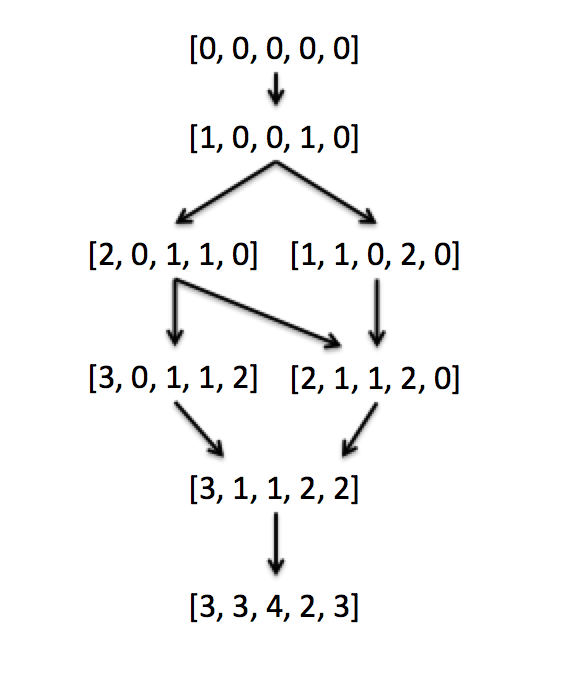
\includegraphics[scale=0.6]{stable_matching_poset.png}
\vspace{-10pt}
\caption{Lattice Representation of Stable Matches}
\label{fig:lattice}
\vspace{-20pt}
\end{wrapfigure}

In this scenario, the man-optimal matching can be expressed as: $[0,0,0,0,0]$. In other words, the man-optimal matching in this case has all men assigned to the first woman on his preference list. If we use the rotation algorithm described above, we can traverse the entire lattice of stable matchings from the man-optimal to the woman optimal. In this case, there are 8 possible stable matchings, shown in the Hasse diagram in Figure~\ref{fig:lattice}.

\subsection{Rotation algorithm}
The algorithm using rotations to traverse through the lattice of all stable matchings is given below:

\begin{enumerate}
    \item Use the Gale-Shapely algorithm to calculate the man-optimal stable matching
    
    \item Use the Gale-Shapely algorithm to calculate the woman-optimal stable matching
    
    \item Use the man-optimal and woman-optimal matchings to identify pairings that are not feasible:
    \begin{enumerate}
        \item For a man $M$, any woman $W$ that occurs in $M$'s preference list prior to $M$'s optimal match or after $M$'s pessimal match is not feasible.
        \item Likewise, for a woman $W$, any man $M$ that occurs in $W$'s preference list prior to $W$'s optimal match or after $W$'s pessimal match is not feasible.
    \end{enumerate}

    \item For each person, build a reduced preference list by taking the full preference list, then for each non-feasible pairing($M_i$, $W_j$), remove $M_i$ from the reduced preference list of $W_j$ and remove $W_j$ from the reduced preference list of $M_i$

    \item Calculate the cumulative $score$ for all people in the man-optimal matching.

    \item Starting with the man-optimal matching, execute the following:

    \item Identify any rotations in the given set. For each rotation found:
    \begin{enumerate}
        \item Take the matching produced by applying the rotation.
        \item If the rotation has been visited already, return.
        \item Calculate the cumulative $score$ for all people in the matching. If the score is the lowest found so far, record the score.
        \item Repeat step 7 with the rotated matching.
    \end{enumerate}
\end{enumerate}

This algorithm was able to calculate optimal matching much more efficiently and handled larger data sets. Still, traversing all possible matchings becomes more and more computationally expensive as the number of pairs grow to more than a thousand. The runtime to perform the rotation matching of large data sets is shown in Table~\ref{tab:resultTimes}. 

(Also, one interesting thing I found is that as the number of pairs goes up, the cumulative score of the optimal match becomes much better than the cumulative score of either the man-optimal or woman-optimal matches. It may be interesting to see how the average equity score / average man/woman optimal score as a function of the number of pairs)

(Another interesting idea, although I don't know if we have any space to discuss, is that you could just traverse down one chain of the lattice and maybe find a reasonably good option without necessarily having to traverse every matching in the lattice)

\section{Results}

As noted above, the brute-force strategy was initially tested, but proved to be too inefficient even on small input data sets, therefore we did not do any performance testing of that method.  However, we did find an alternate method for determining infeasible matchings in Gusfield Irving \cite{gusfield}, in conjunction with with the rotation method.  We implemented both and found the feasible preference list produced using our \emph{heuristics} and their \emph{Non-Feasible Prune} method was the same, but the runtime to generate the list was not the same.

\subsection{Runtime Performance}

For performance testing, the runtime of Gale-Shapley(GS) (for men and women optimal), our Heuristics for pruning feasible matchings, the Non-Feasible Prune method, and the Rotation Matching algorithms were all measured.  The results in Table~\ref{tab:resultTimes} are averages for multiple runs of a set of different input preference lists for each input $n$ size.  Larger inputs were tried, but due to memory constraints and algorithm implementation details, larger than 2000 would not run.

\mytable{Runtime Performance (in msec)}{tab:resultTimes}{%
\begin{tabular}{c|cccc}
     Input $n$ & GS & Heuristic Prune & Non-Feasible Prune & Rotation Matching  \\ \hline
     10 & 0.035 & 0.148 & 0.025 & 0.07 \\
     100 & 2.05 & 4.539 & 2.66 & 25.01 \\ 
     1000 & 254 & 3230 & 908 & 64,147 \\
     2000 & 1336 & 27,382 & 4455 & 762,314 
\end{tabular}
}

\subsection{Fairness Performance}

Insert Table here with fairness metrics

\section{Conclusions}

\begin{thebibliography}{9}
\bibitem{shapely}
  D. Gale and L. S. Shapley Jan 1962,
  \emph{College Admissions and the Stability of Marriage, The American Mathematical Monthly, Vol. 69, No. 1 pp. 9-15}.

\bibitem{gusfield}
  Dan Gusfield and Robert W. Irving,
  \emph{The Stable Marriage Problem: Structure and Algorithms 1989}.

\end{thebibliography}
\end{document}